% !TeX encoding = UTF-8
%% Простая презентация с примером включения программного кода и
%% пошаговых спецэффектов
\documentclass[10pt]{beamer}
\usetheme{SPbAU}
%\useoutertheme{infolines}
\usepackage{fontspec}
\usepackage{xunicode}
\usepackage{xltxtra}
\usepackage{xecyr}
\usepackage{hyperref}

%% Minted для подсветки кода
\usepackage{minted}
\usepackage{listings}

\setminted[kotlin]{xleftmargin=\parindent, linenos, autogobble, frame=lines, escapeinside=\#\#}
\setminted[text]{xleftmargin=\parindent, autogobble, frame=lines, escapeinside=\#\#}

\usepackage{setspace}

\setmainfont[Mapping=tex-text]{DejaVu Serif}
\setsansfont[Mapping=tex-text]{DejaVu Sans}
\setmonofont[Mapping=tex-text]{DejaVu Sans Mono}
\usepackage{polyglossia}
\setdefaultlanguage{russian}
\usepackage{graphicx}
\usepackage{listings}
\lstdefinestyle{mycode}{
  belowcaptionskip=1\baselineskip,
  breaklines=true,
  xleftmargin=\parindent,
  showstringspaces=false,
  basicstyle=\footnotesize\ttfamily,
  keywordstyle=\bfseries,
  commentstyle=\itshape\color{gray!40!black},
  stringstyle=\color{red},
  numbers=left,
  numbersep=5pt,
  numberstyle=\tiny\color{gray},
}
\lstset{escapechar=@,style=mycode}

\newcommand{\code}[1]{\texttt{#1}}

\graphicspath{{img/}}

\definecolor{schema-keyword}{RGB}{0, 0, 128}
\newcommand{\keyword}[1]{\textbf{\textcolor{schema-keyword}{#1}}}

\begin{document}
\title[Поиск списываний в контестах]{Поиск списываний в контестах по программированию с помощью построения графов зависимостей программ}

\author[Анисимова К.В.]{Анисимова Карина Витальевна\\{\footnotesize\textcolor{gray}{научный руководитель: А.В. Садовников}}}
\institute{НИУ ВШЭ - Санкт-Петербург}
\date{19 января 2022 г.}
\frame{\titlepage}

\begin{frame}[fragile]\frametitle{Задача поиска списывания}
\begin{columns}[T]
    \column{0.5\textwidth}
  Программа 1:

  \begin{minted}[fontsize=\small]{cpp}
    #include <iostream>
    using namespace std;
    
    int main() {
        int a, b;
        a = 5;
        b = 4;
        if (a > 4) {
            cout << a - b;
        } else {
            cout << a + b;
        }
        return 0;
    }
  \end{minted}
  
  \column{.02\textwidth}
  	\rule{.1mm}{0.7\textheight}


  \column{0.5\textwidth}
  Программа 2:

  \begin{minted}[fontsize=\small]{cpp}
  #include <iostream>
  using namespace std;
  
  int main() {
      int k = 5;
      int l = 4;
      if (k <= 4) {
          cout << k + l;
      } else {
          cout << k - l;
      }
      return 0;
  }
  \end{minted}
  
\end{columns}
      
  
  
\end{frame}

\begin{frame}[fragile]\frametitle{Задача поиска списывания. Основные модификации}
	\begin{itemize}
		\item Добавление/удаление комментариев
		\item Добавление незначимых строк кода
		\item Переименование
		\item Перестановка операций
		\item Взаимозаменяемые конструкции
		\begin{itemize}
			\item for/while
			\item if/else
		\end{itemize}
	\end{itemize}
\end{frame}


\begin{frame}[fragile]\frametitle{Существующие решения и аналоги}
	\begin{itemize}
		\item Антиплагиат
		\begin{itemize}
			\item проверяет код как обычный текст
		\end{itemize}
		\item SIM
		\begin{itemize}
			\item токенизация
			\item С, Java, Pascal
		\end{itemize}
	    \item Moss
	    \begin{itemize}
	    	\item токенизация
	    	\item С/C++, C#, Java, assembly
	    \end{itemize}
		\item GPLAG
		\begin{itemize}
			\item Program Dependency Graph
			\item Только для Java
			\item Код утерян
		\end{itemize}
	\end{itemize}
\end{frame}

\begin{frame}\frametitle{Program Dependency Graph}
	\begin{definition}
		\textbf{Program Dependency Graph (PDG)} -- представление программы в виде графа. \\
		\textbf{Вершинами} являются базовые выражения. \\
		\textbf{Ребра зависимости по данным} соединяют вершины, в которых используются одинаковые данные. \\
		\textbf{Ребра передачи управления} соединяют две вершины, если контролирующая вершина определяет, будет ли выполняться выражение в зависимой вершине.
	\end{definition}
\end{frame}

\begin{frame}\frametitle{Program Dependency Graph}
	\begin{columns}[C]
		\column{0.7\textwidth}
		\includegraphics[scale=0.4]{pdg_example.png}
		
		\column{.05\textwidth}
		
		\column{0.3\textwidth}
		\centering
		\includegraphics[scale=0.3]{pdg_example2.png}
		
	\end{columns}
\end{frame}

\begin{frame}\frametitle{Постановка цели и задачи}
    \textbf{Цель:} Оценить применимость подхода статьи GPLAG к решению задачи поиска контестного плагиата
    
    \textbf{Задачи:}
    \begin{itemize}
        \item Реализовать алгоритм из статьи GPLAG
        \item Собрать датасет
        \item Провести тестирование и проанализировать работу полученного решения
    \end{itemize}
\end{frame}

\begin{frame}\frametitle{Алгоритм}
\centering
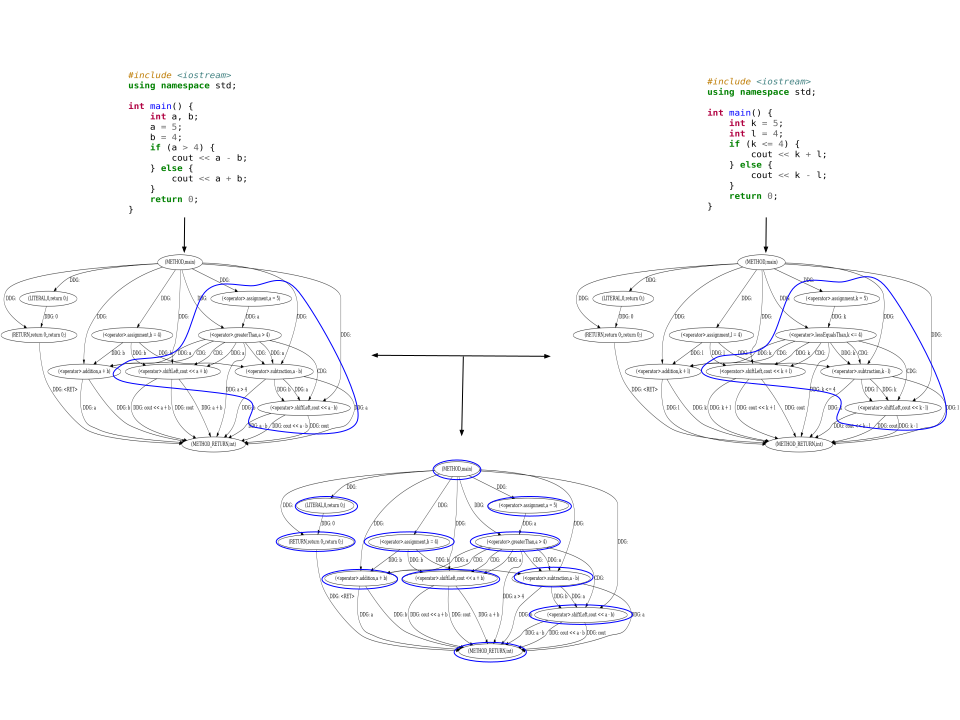
\includegraphics[width=0.8\paperwidth,height=0.8\paperheight]{algo.png}
\end{frame}

\begin{frame}\frametitle{Построение PDG}
    \begin{itemize}
    	\item PROGEX
    	\begin{itemize}
    		\item Парсит только Java, но можно добавлять и свои грамматики
    		\item На практике добавление новой грамматики проблематично
    	\end{itemize}
    	\item TinyPDG
    	\begin{itemize}
    		\item Умеет парсить только Java код
    		\item Добавление новой грамматики не предусмотрено
    	\end{itemize}
        \item Joern
        \begin{itemize}
        	\item Умеет парсить только C/C++ и Java код
        	\item Результат в формате *.dot
        \end{itemize}
    \end{itemize}
\end{frame}
    
\begin{frame}\frametitle{Сравнение графов}
	\begin{columns}[T]
	\column{0.5\textwidth}
		\begin{itemize}
		\item Алгоритмы поиска изоморфизмов типа граф - подграф не подходят
		\item Подграфов в графах слишком много
		\item Нужно учитывать типы вершин и ребер
		\end{itemize}
	
	\column{.02\textwidth}
	\rule{.1mm}{0.7\textheight}
	
	\column{0.5\textwidth}
	\begin{itemize}
	\item Строим подграфы меньшего графа, ищем изоморфизмы вида граф - подграф для всех пар (подграф меньшего графа, больший граф)
	\item Фиксируем размер подграфов: 9 вершин. Предподсчитаем подграфы для тестовых данных.
	\item Сужаем типы вершин до 60 основных
	\end{itemize}
	\end{columns}
 
\end{frame}

\begin{frame}\frametitle{Построение датасета}
	Датасет для оценки способности алгоритма находить плагиат и чувствительности к разным видам модификаций:
	\begin{itemize}
		\item 372 программы из 23 контестов с Codeforces
		\item С помощью инструмента gorshochek построены модификации:
		\begin{itemize} 
			\item Добавление/удаление комментариев
			\item Переименование
			\item Замена взаимозаменяемыех конструкций
		\end{itemize}
		\item Добавлена возможность построения модификации вставки незначимых строк кода в gorshochek
		\item Для каждой программы построен файл с случайным набором модификаций
	\end{itemize}
	
\end{frame}

\begin{frame}\frametitle{Построение датасета}
	Датасет для оценки работы алгоритма в случаях отсутствия плагиата:
	\begin{itemize}
		\item 23 программы, решающих одну и ту же простую задачу
		\item 12 программ, решающих одну и ту же сложную задачу
	\end{itemize}
	
\end{frame}

\begin{frame}\frametitle{Тестирование. Детали}
	\begin{itemize}
		\item Смотрим на количество покрытых вершин
		\item Идеальным результатом считаем покрытие графа при сравнении с собой
		\item Оцениваем метрику похожести
		\item Похожесть = $\frac{\text{Полученное покрытие}}{\text{Максимальное покрытие}}$
	\end{itemize}
    
\end{frame}

\begin{frame}\frametitle{Тестирование. Результаты}
	\begin{columns}[C]
	\column{0.5\textwidth}
	\centering
	\includegraphics[scale=0.25]{res.png}
	
	\column{0.5\textwidth}
	\centering
	\includegraphics[scale=0.25]{res2.png}
	
\end{columns}
	
\end{frame}

\begin{frame}\frametitle{Тестирование. Результаты}
		\begin{columns}[C]
			\column{0.5\textwidth}
			\centering
			\includegraphics[scale=0.27]{res3.png}
			 
			\column{0.5\textwidth}
			\centering
			\includegraphics[scale=0.27]{res4.png}
			
		\end{columns}
	\end{frame}
		
		
\begin{frame}\frametitle{Тестирование. Результаты}
	\begin{columns}[T]
		\column{\textwidth}
		\centering
		\includegraphics[scale=0.26]{res5.png}
	\end{columns}
\end{frame}


\begin{frame}\frametitle{Итоги}
	\begin{itemize}
		\item Реализовала алгоритм из статьи GPLAG
		\item Поддержала гибкость в работе с разными языками программирования
		\item Поддержала гибкость в работе с разными подходами к построению PDG
		\item Собран датасет для оценки возможности применения алгоритма к поиску контестного плагиата
		\item Провела исследование и доказала применимость алгоритма
	\end{itemize}
\end{frame}

\begin{frame}\frametitle{Дальнейшие планы}
    \begin{itemize}
        \item Заменить в системе построение PDG по абстрактному синтаксису на построение PDG по assembler и сравнить эти два подхода
        \item Придумать и применить эвристики для ускорения поиска подграфов и сокращения их количества без сильной потери точности работы алгоритма
        \item Решить проблему нахождения плагиата в случаях популярных паттернов
        
    \end{itemize}
\end{frame}
\end{document}

